\documentclass[conference]{IEEEtran}
\ifCLASSINFOpdf
\else
\fi

\usepackage[utf8]{inputenc}
\usepackage[spanish]{babel}
\usepackage{graphicx}
\graphicspath{ {images/} }
\hyphenation{op-tical net-works semi-conduc-tor}
\begin{document}

\title{Sintetizador de Textos\\ Utilizando Grafos}

\author{

\IEEEauthorblockN{}

\IEEEauthorblockN{Juan Pablo Peñaloza Botero, William Moreno, Johan Sebastian Murillo, Nicolas Miranda}
\IEEEauthorblockA{Pontificia Universidad Javeriana\\
Bogotá, Colombia\\
Email: \{juan-penaloza, williammoreno, johanmurillo, nicolasmiranda\}@javeriana.edu.co}
}
\maketitle

\begin{abstract}
En este documento, presentamos TextRank, un modelo de clasificación basado en gráficos para el procesamiento de texto, y mostramos cómo este modelo se puede utilizar con éxito en aplicaciones de lenguaje natural. En particular, proponemos dos métodos innovadores no supervisados para la extracción de palabras clave y frases, y muestran que los resultados obtenidos se comparan favorablemente con los resultados publicados anteriormente en los puntos de referencia establecidos.
\end{abstract}

\IEEEpeerreviewmaketitle

\section{Introduction}

Algoritmos de clasificación basados en gráficos como los de Kleinberg Algoritmo HITS (Kleinberg, 1999) o Google PageRank (Brin y Page, 1998) han sido exitosos completamente utilizado en el análisis de citas, redes sociales y el análisis de la estructura de enlace de la World Wide Web. Podría decirse que estos algoritmos se pueden destacar como elementos clave del cambio de paradigma desencadenado en el campo de la tecnología de búsqueda web, proporcionando un Mecanismo de clasificación de páginas web que depende del conocimiento colectivo de los arquitectos web en lugar de análisis de contenido individual de páginas web. En resumen, un Algoritmo de clasificación basado en gráficos es una forma de decidir sobre la importancia de un vértice dentro de un gráfico, por al tener en cuenta la información global de forma recursiva de todo el gráfico, en lugar de confiar únicamente en información local específica del vértice. \\
Aplicando una línea de pensamiento similar a gráficos semánticos extraídos de documentos con  lenguaje natural, resulta en un modelo de clasificación basado en gráficos que se puede aplicar a una variedad aplicaciones de procesamiento del lenguaje natural, donde se extrae el conocimiento de un texto completo, se usa para hacer un ranking local y decisiones de selección. Tal clasificación orientada al texto se pueden aplicar a tareas que van desde autoextracción acoplada de frases clave, a sintetización de textos y desambiguación de los sentidos de las palabras (Mihalcea et al., 2004). En este documento, presentamos el gráfico de TextRank- modelo de clasificación basado para gráficos extraídos de textos de lenguaje natural.

\section{Modelo de TextRank}
La idea básica es hacer un modelo de ranking basado en grafo, con votos o recomendaciones.
Cuando un vértice se une a otro tienen un voto, entre mayor sea este voto mayor importancia tiene la conexión, el valor del vértice $V_i$ es definido por el siguiente(Brin and Page, 1998).

$$S(V_i) = (1-d)+d* \sum_{j\varepsilon In(V_i) }\frac{1}{|Out(V_j)|}S(V_j)$$

Donde $In(V_i)$ is el predecesor y $Out(VI)$ es la sucesor, d es el factor de amortiguación que está entre 0 y 1, el valor de d usualmente es 0.85(Brin and Page, 1998) y es el valor que se va a usar en la implementación. \\
Empezando por números arbitrarios asignados a cada nodo del grafo, e iterar hasta que converja en un objetivo dado, después de correr el algoritmo cada vértice va a tener un valor que es la importancia en el grafo, los valores iniciales no afectan los valores finales, esta valor final solo es afectado por el número de iteraciones.

\section{Grafo no Dirigido}
Aunque tradicionalmente se aplica en grafos dirigidos, un algoritmo recursivo de ranking basado en grafo se puede aplicar en un grafo no dirigido, para grafos débilmente conectados, con el número de vértices proporcional al número de aristas, un grafo no dirigido tiene una mayor convergencia en curvas. \\
La Figura 1 muestra la curva de convergencia con un grafo aleatoria con 250 vértices y 250 aristas.
\begin{figure}
  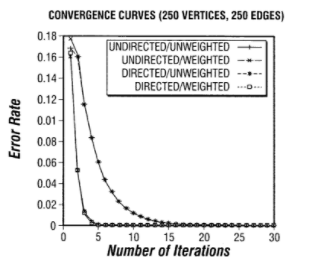
\includegraphics[width=8cm]{figure1.png}
  \caption{Número de Iteraciones}
\end{figure}

\section{Grafo Con Pesos}
En el contexto de Web surfing, es inusual para una pagina incluir múltiples links a otra páginas, y la definición original de PageRank para ranking basado en grafos es asumir un grafo sin pesos.
Sin embargo, en nuestro modelo el grafo se hace con textos que contiene lenguaje natural, y estos incluyen links parciales entre los vértices que son extraídos del texto, es por esto que es muy útil incorporar en el modelo la fuerza de conexión entre los vértices $V_i$ y $V_j$ como el peso de $W_ij$ , agregando en el la arista correspondiente.
Por esta razón se introduce una nueva fórmula que toma en cuenta los pesos de las aristas, esta es:

$$WS(V_i) = (1-d)+d* \sum_{j\varepsilon In(V_i) }\frac{w_{ji}}{\sum_{V_k\in Out(V_j)}w_{jk}}WS(V_j)$$

\section{Texto Como Un Grafo}
Para poder hacer la aplicación del algoritmo de ranking basado en grafos para lenguajes naturales, tenemos que tener un grafo que represente el texto, y conectar las palabras con otras con una relación que tenga significado. Dependiendo de la aplicación la unidad de texto puede tener varios tamaños y las características se pueden agregar en los vértices del grafo, de la misma manera la aplicación dicta el tipo de relación que se utiliza para conectar los vértices. \\
Independientemente del tipo y las característica de los elementos a agregar en el grafo , se puede seguir los siguientes pasos. \\

\begin{enumerate}
  \item Identificar las unidades de texto que mejor definan la tarea, y agregar estos en los vértices del grafo.
  \item Identificar la relación que hay en esas unidades de texto, y usar esas relaciones para hacer las aristas entre los vértices del grafo, las aristas pueden ser dirigidas o no dirigidas y tener peso o no.
  \item Iterar el algoritmo de ranking basado en grafo hasta converger.
  \item Ordenar los vértices basados en el valor final.
\end{enumerate}

\section{Extracción de Palabras Claves}
La tarea de una aplicación de extracción de palabras clave es identificar automáticamente en un texto un conjunto de términos que mejor describa el documento. Dichas palabras clave pueden constituir entradas útiles para construir un índice automático para una colección de documentos, pueden usarse para clasificar un texto o pueden servir como un resumen conciso para un documento dado. Además, se puede utilizar un sistema para la identificación automática de términos importantes en un texto para el problema de la extracción de terminología y la construcción de diccionarios específicos de dominio.\\
En esta sección, informamos sobre nuestros experimentos en la extracción de palabras clave usando TextRank, y mostramos que el modelo de clasificación basado en gráficos supera a los mejores resultados publicados en este problema. Similar a (Hulth, 2003), estamos evaluando nuestro algoritmo de extracción de palabras clave de resúmenes, principalmente con el propósito de permitir una comparación directa con los resultados que informa con su sistema de extracción de frases clave. Tenga en cuenta que el tamaño del texto no es una limitación impuesta por nuestro sistema, y se esperan resultados similares con TextRank aplicado en textos completos.\\

\section{TextRank para la Extracción de Palabras Claves }
El resultado final esperado para esta aplicación es un conjunto de palabras o frases que son representativas de un texto en un idioma natural dado. Por lo tanto, las unidades a clasificar son secuencias de una o más unidades léxicas extraídas del texto, y representan los vértices que se agregan al gráfico de texto. Cualquier relación que se pueda definir entre dos unidades léxicas es una conexión potencialmente útil (borde) que se puede agregar entre dos vértices. Estamos utilizando una relación de ocurrencia conjunta, controlada por la distancia entre las ocurrencias de palabras: dos vértices se conectan si las unidades léxicas correspondientes ocurren simultáneamente dentro de una ventana de palabras máximas, donde se puede establecer desde 2 hasta 10 palabras Los enlaces concurrentes expresan las relaciones entre los elementos sintácticos y, de forma similar a los enlaces semánticos encontrados útiles para la tarea de desambiguación de los sentidos verbales (Mihalcea et al., 2004), representan los indicadores de cohesión para un texto dado.\\
El algoritmo de extracción de palabras clave de TextRank no está supervisado por completo y procede de la siguiente manera. En primer lugar, el texto se tokeniza y se anota con etiquetas de parte de la palabra, un paso de preproceso requerido para permitir la aplicación de filtros sintácticos. Para evitar el crecimiento excesivo del tamaño del gráfico agregando todas las combinaciones posibles de secuencias que constan de más de una unidad léxica (ngramos), consideramos que solo palabras sueltas son candidatas para agregarlas al gráfico, y las palabras clave de varias palabras finalmente se reconstruirán en la fase de post-procesamiento	\\

\section{Evaluación}
TextRank logra la máxima precisión y la medida F en todos los sistemas, aunque la recuperación no es tan alta como en los métodos supervisados - pos-utilizando TextRank o aprendizaje supervisado (Hulth, 2003) posiblemente debido a la limitación impuesta por nuestro enfoque sobre el número de palabras clave seleccionadas, que no se realiza en el sistema supervisado. Una ventana más grande no parece ayudar; por el contrario, cuanto mayor sea la ventana, menor será la precisión, probablemente explicada por el hecho de que una relación entre palabras que están más separadas no es lo suficientemente fuerte como para definir una conexión en el texto
\begin{figure}
  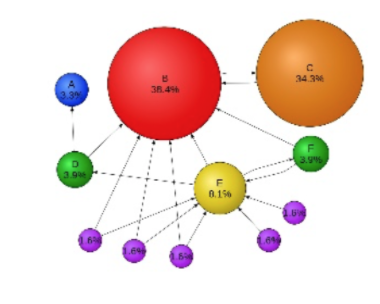
\includegraphics[width=8cm]{figure2.png}
  \caption{Modelo de un texto como un grafo}
\end{figure}
Use el Pagerank para calificar las oraciones en el gráfico. \\
Clasifique las oraciones con la suposición subyacente de que las "oraciones resumidas" son similares a la mayoría de las oraciones. \\

\section{Extracción de Frases}
Otra aplicación de TextRank, consiste en la extracción de frases para el resumen automático. En la extracción de palabras clave, las piezas fundamentales eran palabras pero al ahora tratar con oraciones, nuestra unidad será una oración completa. TextRank ayuda en este tipo de aplicaciones al permitir una clasificación sobre unidades de texto que se calcula de forma recursiva en función del texto.

\section{TextRank Para la Extracción de Frases}
Para aplicar TextRank, primero necesitamos construir un grafo asociado con el texto, donde los vértices del grafo sean representativos de las unidades que se clasificaran. Para esto en cada vértice no existirán palabras como en la extracción de palabras sino frases como ya lo mencionamos anteriormente. La relación que usaremos en este caso será diferente y se relaciona si existe una “similitud” más no una coincidencia. Esta similitud será medida al superponer dos frases y observar su contenido en común y se tendrá en cuenta el número de palabras comunes o tambien se podrian aplicar filtros sintácticos para clasificar las palabras según su sintaxis. \\
Después de aplicar el algoritmo las frases se ordenan por puntaje y las mejores puntuaciones serán las incluidas en el resumen.

\section{¿Por Qué TextRank Funciona? }
Intuitivamente, TextRank funciona bien porque no sólo se basan en el contexto local de una unidad de texto (vértice), sino que toma en cuenta la información recurrente extraída de todo el texto (el gráfico). A través de los gráficos, TextRank identifica las conexiones entre varias entidades en una texto, y pone en práctica el concepto de recomendación. Una unidad de texto recomienda otro texto relacionado unidades, y la fuerza de la recomendación es recursivamente calcula en base a la importancia de la unidades que la recomendación. Por ejemplo, en la aplicación de extracción frase clave, co-produciendo palabras recomendadas entre sí, y es el contexto común que permite la identificación de conexiones entre las palabras en el texto. En el proceso de la identificación de frases importantes en un texto, una frase recomienda otra frase que ocupa similares conceptos que son útiles para la comprensión generalizando el texto. Las frases que son altamente recomendadas por otras frases en el texto es probable que se ser más informativo para el texto dado, y estará Por lo tanto, dada una puntuación más alta.

\section{Conclusion}
En el presente trabajo, hemos introducido TextRank modelo basado en grafos de clasificación basado en el procesamiento de textos, y cómo puede ser utilizado con éxito para el lenguaje natural. En particular, hemos propuesto y evaluado un enfoque innovador para la extracción de palabras claves de un texto utilizando métodos no supervisados, y demostró que la precisión alcanzada por TextRank en estas aplicaciones es competitivo con algoritmos del estado del arte. Un aspecto importante de TextRank es que no requiere conocimiento de lingüística profunda, ni dominio o un lenguaje específico, lo que hace que sea muy portátil a otros dominios, géneros o idiomas.

\begin{thebibliography}{1}
\bibitem{IEEEhowto:kopka}
S. Brin and L. Page. 1998. The anatomy of a large-scale hyper- textual Web search engine. \emph{Computer Networks and ISDN Systems, 30(1–7).}

\bibitem{IEEEhowto:kopka}
DUC. 2002. Document understanding conference 2002. http://www-nlpir.nist.gov/projects/duc/.

\bibitem{IEEEhowto:kopka}
E. Frank, G. W. Paynter, I. H. Witten, C. Gutwin, and C. G. Nevill-Manning. 1999. Domain-specific keyphrase extrac- tion. \emph{In Proceedings of the 16th International Joint Confer- ence on Artificial Intelligence.}

\bibitem{IEEEhowto:kopka}
C.Y. Lin and E.H. Hovy. 2003. Automatic evaluation of summaries using n-gram co-occurrence statistics. \emph{In Proceedings of Human Language Technology Conference (HLT-NAACL 2003), Edmonton, Canada, May.}

\bibitem{IEEEhowto:kopka}
P. Turney. 1999. Learning to extract keyphrases from text. Technical report, National Research Council, Institute for Information Technology.

\bibitem{IEEEhowto:kopka}
R. Mihalcea. 2004. Graph-based ranking algorithms for sentence extraction, applied to text summarization. \emph{In Proceedings of the 42nd Annual Meeting of the Association for Computational Lingusitics (ACL 2004) (companion volume), Barcelona, Spain.}

\bibitem{IEEEhowto:kopka}
R. Mihalcea, P. Tarau, and E. Figa. 2004. PageRank on semantic networks, with application to word sense disambiguation. \emph{In Proceedings of the 20st International Conference on Computational Linguistics (COLING 2004), Geneva, Switzerland.}

\end{thebibliography}

\end{document}
